% paper-ipccc.tex --- IPCCC (IEEE conference) submission version of HPCC-FS.
% Generated alongside paper.tex (the acmart original, which stays canonical).
% Compile: latexmk -pdf paper-ipccc
\documentclass[conference]{IEEEtran}
\IEEEoverridecommandlockouts
\usepackage{booktabs}
\usepackage{graphicx}
\usepackage[caption=false,font=footnotesize]{subfig}
\usepackage{xcolor}
\usepackage{microtype}
\usepackage{url}
\usepackage{amsmath}
\usepackage{algorithm}
\usepackage{algpseudocode}
\usepackage{cite}
\usepackage{xspace}
\graphicspath{{figures/}}
\newcommand{\hpccfs}{\textsc{RDMA-RCP}\xspace}
% acmart-style run-in bold paragraphs (IEEEtran's \paragraph is a numbered sectioning level)
\renewcommand{\paragraph}[1]{\par\smallskip\noindent\textbf{#1}\hspace{0.5em}\ignorespaces}

\begin{document}

\title{Multi-Bottleneck Fairness on RDMA Fabrics: An Empirical Study of Deployable
Congestion Control and an RCP Service Mode over In-Network Telemetry}

\author{
\IEEEauthorblockN{Haoyu Wang\IEEEauthorrefmark{1}, Bo Sheng\IEEEauthorrefmark{1}, Zerin Shaima Meem\IEEEauthorrefmark{2}, Xiaoqian Zhang\IEEEauthorrefmark{2}}
\IEEEauthorblockA{\IEEEauthorrefmark{1}University of Massachusetts Boston, Boston, MA, USA \quad \{haoyu.wang001, bo.sheng\}@umb.edu}
\IEEEauthorblockA{\IEEEauthorrefmark{2}University of Nebraska Omaha, Omaha, NE, USA \quad \{zmeem, xiaoqianzhang\}@unomaha.edu}
}

\maketitle

\begin{abstract}
Modern datacenter traffic increasingly crosses several contended links in series, yet deployable
RDMA congestion control is evaluated almost exclusively on single-bottleneck benchmarks. We
present an empirical study of multi-bottleneck fairness on lossless RDMA fabrics. On a
parameterized parking-lot benchmark with a fluid max-min oracle, \emph{every} deployable scheme
we test is unfair to the multi-bottleneck flow --- DCQCN $1.7$--$2.3\times$, TIMELY
$1.8$--$2.0\times$, DCTCP $1.6$--$1.8\times$, HPCC $1.9$--$2.0\times$ --- growing with
bottleneck count and robust to start-time jitter. For HPCC we localize the mechanism: near-winner-take-all
collapse to ${\sim}0.4$ Gbps. Six sender-only corrections fail --- including a sender-side mirror of RCP driven by the
same INT signals --- and so does per-flow fair queueing under stock senders ($1.97\times$): the
obstacle is where the rate state \emph{lives}. Independently maintained copies of an
explicit-rate recursion preserve arrival-history asymmetry indefinitely; the same recursion on
one shared per-link register erases it. Placing that register at the switch --- \hpccfs, an RCP
service mode carried in one 64-bit INT field with three words of mutable state per port ---
restores the max-min allocation (penalty ${\approx}1.005\times$, every flow within
$5$--$13\%$ of its oracle FCT) with zero PFC in every fairness experiment, rate-only or with a
canonical $cwnd = R \cdot RTT$ window, and cuts a ring-collective coflow's completion time by
$18$--$23\%$ at every seed tested ($18\%$ with the INT header padded to stock size). We also measure the
deployment boundary: RCP-mode and HPCC traffic do not coexist fairly on a shared link, even
under a weighted-DRR reservation, because both classes' control signals remain port-global; we
therefore position \hpccfs as a \emph{fabric-wide} (or isolated-service) mode. Stock HPCC's code
path remains byte-for-byte unchanged.
\end{abstract}

\begin{IEEEkeywords}
datacenter networks, congestion control, RDMA, in-network telemetry, max-min fairness, RCP
\end{IEEEkeywords}


% ============================================================================
\section{Introduction}
% ============================================================================

HPCC~\cite{li2019hpcc} and its derivatives represent the state of the art in datacenter RDMA
congestion control: the switch stamps raw per-hop state into INT headers, and the sender computes
a precise utilization estimate toward a target $\eta$. On the canonical single-bottleneck
benchmarks HPCC matches or beats DCQCN, TIMELY, and DCTCP on flow completion time and queueing
--- and that is where deployable RDMA congestion control is, almost exclusively, evaluated.

Modern datacenter traffic, however, increasingly crosses \emph{several contended links in
series}: cross-pod ML collectives, disaggregated memory and storage, multi-tenant aggregation
and core layers. The practical stake is concrete: a collective completes when its
\emph{slowest} flow completes, and the slowest flows are precisely the cross-fabric,
multi-bottleneck ones. On a 16-flow ring-collective coflow over a $k{=}4$ fat-tree, we measure stock
HPCC inflating job completion time by ${\sim}27\%$ over what max-min allocation delivers ---
at every ECMP hash seed we test (\S\ref{sec:jct}). Whether deployable RDMA congestion control
is fair to such traffic has not been carefully measured. This paper measures it.

Max-min fairness is a policy choice, not a universal congestion-control objective; our claims
target traffic classes whose completion is gated by multi-bottleneck flows, and \S\ref{sec:scope}
delimits where it is the wrong target. We proceed with a deterministic, oracle-grounded
methodology. Our simulator \emph{is} the original HPCC authors' ns-3 code base, upgraded to a
tagged modern release (ns-3.45): the changes are interface-level --- build-system, header, and
deprecated-API adaptations --- while the congestion-control logic, switch datapath, and wire
formats are the original code (one latent field-initialization bug, exposed only by the 376-node
topology, is fixed and documented). We validated the upgrade by reproducing the original paper's
baseline comparisons across five schemes and two production workloads (\S\ref{sec:eval}); the
reproduction record and raw results are public. The measurements here are therefore produced by
the original HPCC implementation's logic, not a re-implementation. Our findings:

\begin{enumerate}
\item \textbf{The failure spans every scheme we evaluate, and we characterize HPCC's instance}
(\S\ref{sec:bg}, \S\ref{sec:endemic}). Every deployable scheme we test is unfair to the
multi-bottleneck flow --- DCQCN $1.70$--$2.32\times$, TIMELY $1.83$--$2.01\times$, DCTCP
$1.61$--$1.78\times$, HPCC $1.90$--$1.96\times$ at $N = 2$--$4$ --- all growing with bottleneck
count, and robust to start-time jitter. For HPCC we isolate the mechanism: the failure is
\emph{near-winner-take-all} (the long flow collapses to ${\sim}0.4$ Gbps against ${\sim}23$ Gbps
competitors; $3.5\times$ for small flows), RTT-independent, immune to HPCC's own per-hop
multi-rate mode and to INT compression (PINT), and compounded past four bottlenecks by a
wire-format cap ($\texttt{maxHop}=5$) that corrupts the control input. A single-bottleneck
control ($N{=}1$: $1.10$--$1.39\times$ pairwise spread, direction set by arrival order)
separates HPCC's baseline rate lottery from the systematic multi-bottleneck penalty on top.

\item \textbf{Private replication of the fair-rate computation cannot close the gap ---
shared placement can} (\S\ref{sec:senderonly}). We evaluate six sender-only designs: five
heuristics, plus the most direct variant --- a full sender-side mirror of the RCP recursion
driven by the same INT-visible inputs the switch would use. The mirror still fails
($1.56\times$ even with synchronized starts; $1.65\times$/$0.81\times$ under staggered
arrival, the \emph{direction} set by arrival order), while the identical law at the switch
holds ${\approx}1.0\times$; per-flow fair queueing under stock senders leaves the gap intact
too ($1.97\times$). The mechanism is history: independently maintained rate state preserves
arrival-order asymmetry indefinitely, while a shared per-link register eliminates that history
dependence --- evidence about explicit-rate state placement, not a formal impossibility for
every endpoint law (\S\ref{sec:senderonly}).

\item \textbf{An RCP service mode over INT restores max-min, verified end to end}
(\S\ref{sec:design}, \S\ref{sec:eval}). \hpccfs carries a switch-computed RCP fair rate in one
64-bit INT field with three words of mutable state per egress port, alongside
byte-for-byte unchanged stock HPCC. It reaches penalty ${\approx}1.005\times$ across bottleneck
counts, asymmetric sizes, staggered and jittered starts, and ECMP hash seeds, with zero PFC in
every fairness experiment --- operating rate-only or with a canonical RCP window
($cwnd = R \cdot \mathrm{baseRTT}$), and cutting ring-collective coflow JCT by $18$--$23\%$
at every seed tested ($18\%$ under a byte-identical INT header). We equally report its deployment boundary: sharing a link with stock HPCC serves neither
class, even under a weighted-DRR reservation, because both controllers read port-global
telemetry (\S\ref{sec:integration}) --- a fabric-wide or isolated-service mode. The mechanism
is RCP; we claim the measurement study and the placement result, not a new control law.
\end{enumerate}

\paragraph{Artifacts.} The implementation, the topology/workload generators, the max-min oracle,
and deterministic scripts that regenerate the figures (\texttt{make\_figures.py}) and the
ablation/sensitivity/baseline tables (\texttt{run\_sensitivity.py}) from source are available in our
artifact-review repository.\footnote{\url{https://github.com/UNOCourseDemo/hpcc-fs}}

% ============================================================================
\section{Background and Motivation}
\label{sec:bg}
% ============================================================================

\subsection{HPCC, briefly}

HPCC's per-hop utilization estimate for hop $i$ is
\begin{equation}
u_i = \frac{\mathit{txRate}_i}{C_i} + \frac{\min(\mathit{qlen}_i, \mathit{qlen}_i^{\mathrm{prev}}) \cdot \mathit{maxRate}}{C_i \cdot W}
\end{equation}
where the first term reflects bandwidth utilization and the second is a queue-drain term that
keeps standing queues bounded. In single-rate mode the sender takes $U = \max_i u_i$, smooths
it over the base RTT, and applies
\[
\mathit{new\_rate} = \begin{cases} \mathit{curRate} / \max c + R_{AI} & \max c \ge 1 \\ \mathit{curRate} + R_{AI} & \text{otherwise} \end{cases}
\]
with $\max c = U / \eta$. The window $W$ is sized to $m_{win} \cdot \mathit{rate} / \mathit{NIC\_line}$
under \texttt{var\_win}.

\subsection{The multi-bottleneck parking lot}

The \emph{parking lot} is a classic congestion-control fairness
benchmark~\cite{bertsekas1992data, katabi2002xcp}. Because every link is equally contended, the
\emph{max-min fair} allocation~\cite{bertsekas1992data} gives every flow an equal share, so the
long flow should run exactly as fast as each cross flow despite traversing many contention points
rather than one. The parking lot therefore isolates the multi-bottleneck fairness question in its
simplest form, with no confounding asymmetry in link capacity or hop count of the competitors.
One control is essential before reading any deviation as a multi-bottleneck effect: on a
\emph{single} shared bottleneck ($N{=}1$) with two symmetric 50\,MB flows, stock HPCC already
allocates unequally ($37.20$ vs $26.72$\,ms, a $1.39\times$ spread), while \hpccfs equalizes
them exactly ($33.89$ vs $33.89$\,ms). Stock HPCC therefore carries a baseline rate unfairness
between symmetric flows; the multi-bottleneck penalty we characterize is the \emph{additional}
deviation on top of it, growing to $1.90$--$1.96\times$ at $N = 2$--$4$.

We construct a parameterized parking-lot benchmark with $N$ inter-switch bottleneck links
(25 Gbps each) and 100 Gbps host links (Figure~\ref{fig:topo-parking}). One ``long'' flow
traverses all $N$ bottlenecks; one ``cross'' flow traverses each single bottleneck. Flows are
50 MB by default and start simultaneously at $t = 0$. With two flows sharing each 25 Gbps link,
the max-min fair rate is 12.5 Gbps for every flow. All experiments are deterministic: each
configuration produces byte-identical artifacts across repeated runs (verified).

\begin{figure*}[t]
\centering
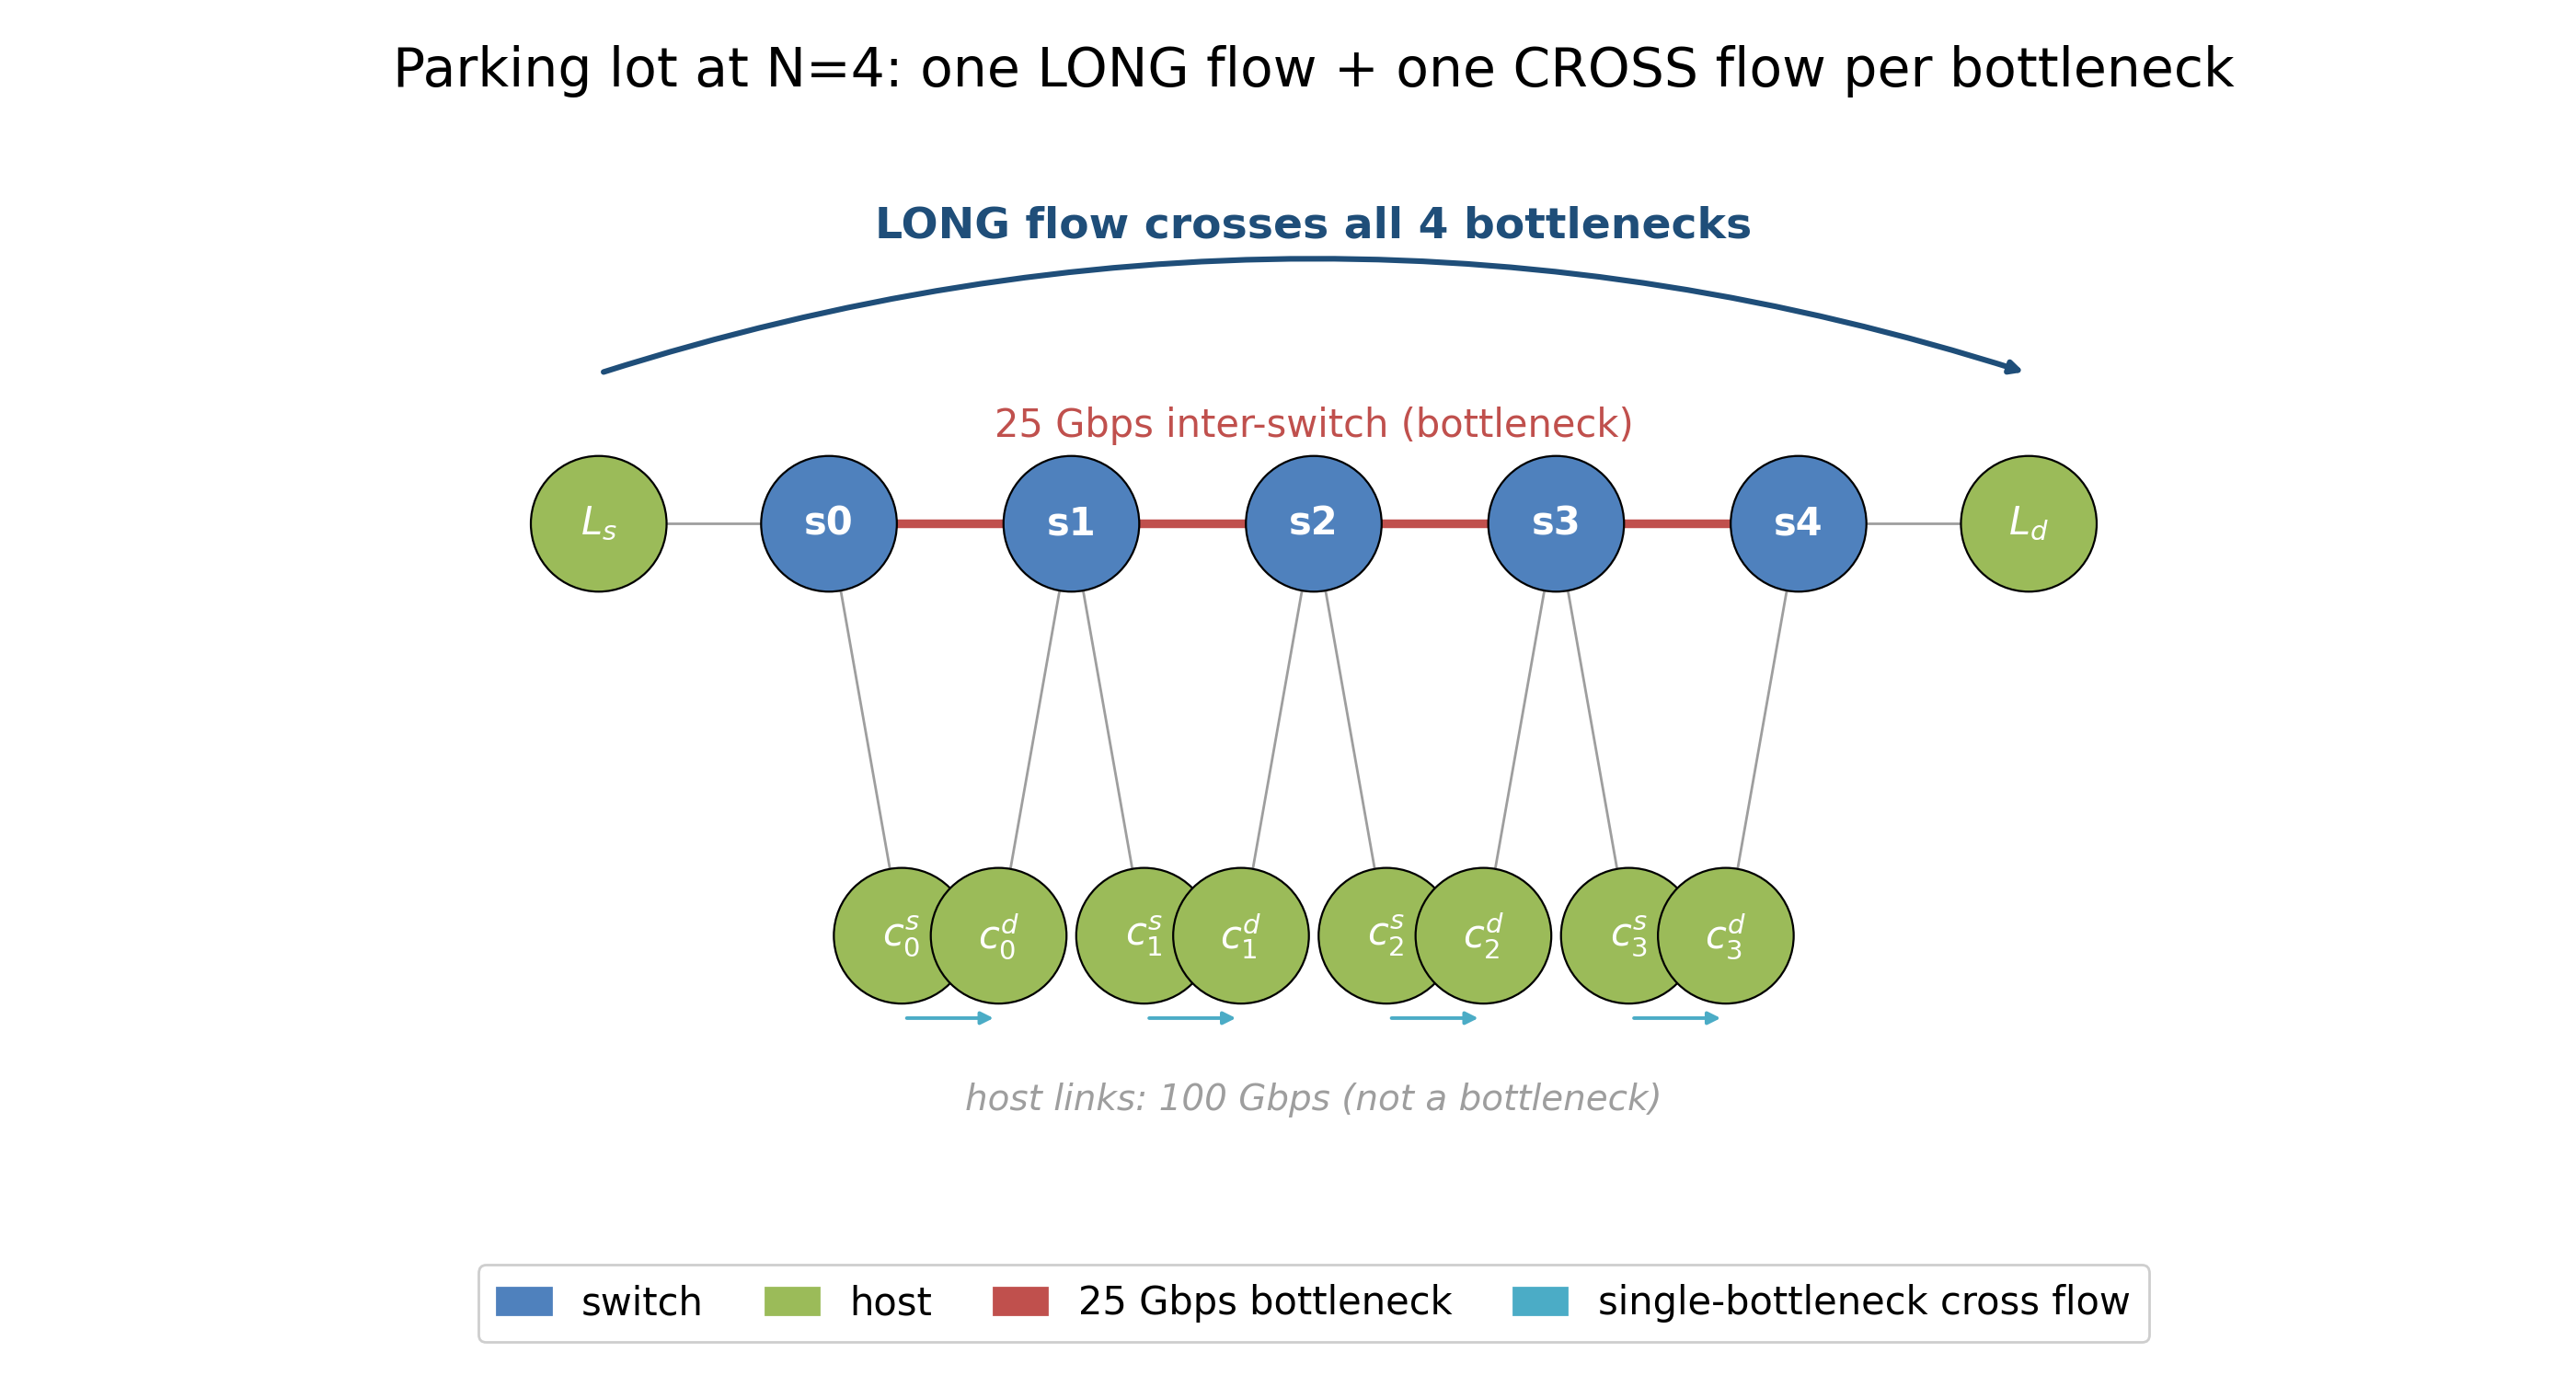
\includegraphics[width=0.82\textwidth]{fig_topo_parking.png}
\caption{Parking-lot benchmark at $N = 4$. The long flow $L_s {\to} L_d$ crosses every
bottleneck; each cross flow $c_i^s {\to} c_i^d$ traverses exactly one. Host links are not
bottlenecks.}

\label{fig:topo-parking}
\end{figure*}

\paragraph{Metric.} We compare each flow's actual flow completion time (FCT) against an
idealized \textbf{fluid max-min oracle} --- a continuous bandwidth-sharing model with no protocol
dynamics (no slow start, no queueing, no convergence delay) in which the bandwidth is allocated
max-min fairly at every instant. We compute the allocation by \emph{progressive
filling}~\cite{bertsekas1992data}: all active flows raise their rate in lockstep until some link
saturates; the flows crossing that link are frozen at their current rate; and the process repeats
on the remaining flows until every flow is frozen. Because flows complete and depart over time, we run it \emph{event-driven} ---
recomputing the allocation at each flow completion --- so the oracle FCT correctly accounts for
the bandwidth freed as short flows finish. The oracle is therefore the best FCT any
rate-allocation scheme could achieve under max-min fairness, and is exact for our fluid
topologies. The headline metric is the \textbf{unfairness ratio}
$\max_{\text{path}}\mathit{FCT} / \mathrm{mean}(\text{short-path FCT})$; the oracle's value is
$1.0$ for equal-size, simultaneous flows.

\subsection{Findings F1--F4: characterizing the gap}

\paragraph{Magnitude.} Stock HPCC's unfairness ratio at $N \in \{2, 3, 4\}$ is $1.90$, $1.92$,
$1.96$: the multi-bottleneck flow's FCT is roughly twice that of single-bottleneck competitors.
\textbf{There is a non-monotonic regime change at $N \ge 5$}, where the long flow becomes
favored ($0.51\times$); this turns out to be an INT-overflow artifact at $\texttt{maxHop} = 5$
and we exclude $N \ge 5$ from the rest of this paper's stock comparisons
(Figure~\ref{fig:nsweep}).\footnote{The 5-hop cap is HPCC's original wire format, not an
artifact of our ns-3 upgrade: the reference simulator hard-codes $\texttt{maxHop}=5$ in its INT
header~\cite{hpccrepo}, consistent with the paper's 42-byte worst-case INT overhead (five
8-byte hop records). Conversely, a parking-lot path at $N \le 4$ traverses at most five
switches --- \emph{within} the INT budget --- so the retained $N = 2$--$4$ measurements are
structurally free of the overflow.}

\paragraph{Robustness.} Size and start-time perturbations give $1.81$--$3.53\times$
(Figure~\ref{fig:robustness}), worst ($3.5\times$) when the multi-bottleneck flow is small ---
the latency-sensitive RPC case. \emph{Multi-rate HPCC} (per-hop EWMA, $\min_i Rc_i$) helps but
does not fix it ($1.44$--$1.75\times$, growing with $N$). \emph{RTT-equalization rules out RTT
bias:} the penalty stays ${\sim}1.9\times$ across a $4.5\times$ sweep of cross-flow RTTs
(cross-flow RTT up to $1.8\times$ the long flow's).

\paragraph{Trace diagnosis.} At $N = 4$ (Figure~\ref{fig:rate-trace} left) the long flow
collapses to ${\sim}0.38$ Gbps while the four cross flows hold ${\sim}23.2$ Gbps each for the
entire 19 ms contention window, with zero PFC and zero loss --- \emph{winner-take-all}: at every
shared link the local single-bottleneck flow wins and the long flow is squeezed. This is an
equilibrium, not a transient: with 500 MB flows ($10\times$ the contention, ${\sim}7{,}000$
RTTs) the ratio is $1.975\times$, the long flow flat at $0.39$ Gbps for 150 ms.

% ============================================================================
\section{The Limits of Sender-Side Control}
\label{sec:senderonly}
% ============================================================================

A natural first design instinct --- and the one our project explored exhaustively --- is to
keep all state and computation at the sender, since HPCC's value proposition is its stateless
switch design. We evaluated six sender-only correction variants behind a new \texttt{mb\_mode}
config knob, on top of unchanged HPCC; the \texttt{mb\_mode = 0} path is byte-identical to
stock HPCC (verified). Five are small heuristic changes to \texttt{UpdateRateHp}; the sixth is
the most direct: a full sender-side mirror of the RCP recursion.

\subsection{Five heuristic variants}

The five heuristics attack different levers of HPCC's update law: a $k$-aware additive boost
scaled by the congested-hop count ($1.63\times$, the best case, at $\gamma{=}50$); a debiased
max/mean blend of per-hop $u_i$ ($1.95\times$ --- the $u_i$ are nearly equal here); a
responsibility-weighted MD ($1.89\times$) and a $k$-th-root MD ($1.92\times$) --- the MD
branch barely fires at $\eta$-hold; and a share-aware additive increase on every flow
($1.71\times$). Stock is $1.96\times$; the target is $1.0$.

\subsection{Isolating placement: identical observations, private vs.\ shared state}
\label{sec:isolate}

We first isolate placement cleanly: a deterministic fluid model of one link where every
controller receives the exact same $(y, q)$ observations at the same update instants, with
identical rule, gains, and initialization --- only the \emph{location of the recursion state}
differs (\texttt{run\_consistency.py}; flow 2 arrives at $t{=}5$\,ms). Shared register: the
late arrival inherits the evolved state; $12.5/12.5$ Gbps. Private, synchronized: identical
trajectories, equally fair --- the information is sufficient. Private, staggered: the newcomer
initializes fresh, both multiply by the same factor thereafter, and the ratio freezes at exactly
$2{:}1$ ($16.67$/$8.33$ Gbps) forever. The one thing a sender cannot replicate is the register's
\emph{history}.

\subsection{The full stack: a virtual-RCP mirror}
\label{sec:vrcp}

The fluid model isolates the mechanism; \texttt{mb\_mode 6} confirms it in the full stack.
RCP's inputs --- $C$, $y$, $q$ --- are all sender-visible in HPCC's INT record, so the sender
runs the switch's recursion \emph{privately}: per hop, a virtual fair rate $\hat R_i$ updated by
the identical rule from the flow's own INT samples, sending at $\min_i \hat R_i$ (same gains,
same $R_0 = C/2$, the sender's own base RTT as control interval). Beyond the fluid model's
arrival asymmetry, the real stack adds per-flow sampling and feedback-delay asymmetry --- which
is why the mirror falls short even under synchronized starts.

Table~\ref{tab:vrcp}: the mirror reaches only $1.56$--$1.65\times$ (direction set by
arrival order), while the identical law at the switch holds $1.003$--$1.008\times$
throughout.

\begin{table}[t]
\caption{Same control law, same INT-visible inputs, different placement ($N{=}4$ parking
lot; ``late'' = $+5$\,ms start).}
\label{tab:vrcp}
\centering\small
\begin{tabular}{lccc}
\toprule
 & synchronized & long late & crosses late \\
\midrule
switch (shared per-port $R$) & $1.005\times$ & $1.008\times$ & $1.003\times$ \\
sender (private $\hat R$)    & $1.560\times$ & $1.654\times$ & $0.813\times$ \\
\bottomrule
\end{tabular}
\end{table}

\subsection{The structural reason: consistency, not information}

Two observations explain the pattern. \emph{First, the $\eta$-hold equilibrium:} once the
contended links settle at target utilization $\eta$, HPCC's multiplicative term
$1/\max c \approx 1$ and every flow holds its current rate --- whoever grabbed more at startup
keeps it. Additive nudges (modes 1, 5) are orders of magnitude too slow relative to flow
lifetimes (our 200\,ms runs are ${\sim}10^4$ RTTs and they never converge), and MD-side
modifications (modes 3, 4) rarely fire at the hold point.

\emph{Second --- what mode 6 isolates --- private explicit-rate state preserves history.} The
information needed to compute the fair share is sender-visible; what a private copy of the
recursion cannot reproduce is the shared register's evolved \emph{history}. A multiplicative
update on independently initialized state preserves the ratio set at arrival forever
(\S\ref{sec:isolate}); the same update on one shared per-link register makes every flow ---
incumbent or newcomer --- adopt the same $R$ within one RTT, eliminating the history
dependence. This is why RCP~\cite{dukkipati2006fct,dukkipati2008rcp} and
XCP~\cite{katabi2002xcp} place the computation in the network. The scheduling side
corroborates it: per-flow equal-weight DRR queues at every port under unchanged HPCC senders
leave the penalty at $1.97\times$ (\texttt{run\_round3.py}) --- a work-conserving scheduler
cannot assign bandwidth the window-limited long flow never offers; the correction must reach
the \emph{signal} the sender obeys. Our claim is thus scoped: for private reconstructions of
an explicit fair rate, placement of the state is decisive --- six sender-side designs fail
while the identical law at the switch succeeds. It is not a formal impossibility for every
endpoint law: contractive designs (AIMD-style convergence toward equal windows) escape the
history argument in principle, though the AIMD-flavored schemes we measure (DCQCN, DCTCP)
still show $1.6$--$2.3\times$ (\S\ref{sec:endemic}).

% ============================================================================
\section{RDMA-RCP Design}
\label{sec:design}
% ============================================================================

The empirical and structural arguments of \S\ref{sec:senderonly} motivate a design that (a)~makes the \emph{dominant} flows yield rather than merely nudging the victims, and (b)~places a fair-rate
\emph{signal} at the switch, since the sender cannot recover the fair share from a load signal
alone. We do not have the switch count flows and divide; instead each port runs a standard RCP control
law on aggregate load and queue (below) whose fixed point \emph{is} the max-min fair rate
$C/N$. We take the most
minimal mechanism consistent with these constraints, packaged as an \emph{operating mode}
alongside stock HPCC on the same INT transport, selected per fabric or isolated slice
(\S\ref{sec:integration}).

\paragraph{Background: RCP} The Rate Control Protocol (RCP)~\cite{dukkipati2006fct,dukkipati2008rcp} is a
router-assisted congestion control in which each link advertises a \emph{single} rate $R$ to
\emph{all} flows crossing it, holding no per-flow state. The key point is that $R$ is not an
aggregate budget for the link; it is the rate \emph{each individual flow} should send at, such
that when all of them do, the link is exactly full and shared equally. Routers stamp $R$ into
passing packets and each flow sends at the minimum $R$ along its path. With $N$ flows each
sending $R$, the controller drives $N R \to C$ (idle link $\Rightarrow$ $R$ rises; standing
queue $\Rightarrow$ $R$ falls), so at equilibrium $R \approx C/N$ --- the max-min
(processor-sharing) share of the flows bottlenecked there, tracked \emph{without counting $N$}:
as flows arrive or leave, $R$ self-adjusts. RCP thus supplies exactly the missing ingredient from
\S\ref{sec:senderonly}: a fair-share signal computed where the flow count is implicitly observable
(the link), not at the sender. \hpccfs runs this control law once per egress port and carries its
$R$ in the INT header; a flow's path-minimum $R$ approximates network-wide max-min fairness (within $1.2\%$ of the oracle on our benchmarks), since a
flow bottlenecked elsewhere contributes less load here and the loop hands the slack to the rest.

\subsection{The mechanism}

The entire protocol is Algorithms~\ref{alg:switch} and~\ref{alg:sender}. The switch maintains one
scalar fair rate per egress port and stamps the path-minimum into a single header field; the
sender reads that field from the returning ACK and adopts it. No per-flow switch state, no
per-hop record, no receiver changes.

\begin{algorithm}[t]
\caption{\hpccfs switch --- per egress port $j$}
\label{alg:switch}
\begin{algorithmic}[1]
\State \textbf{State} $R_j$ (fair rate), $t_j$ (last update), $B_j$ (txByte snapshot)
\State \textbf{Const} $C_j$ link capacity; $\alpha{=}0.4$, $\beta{=}0.226$; $d$ control interval ($\approx$ RTT); $R_{\min}$
\Procedure{OnDequeue}{$pkt$, $j$}\Comment{every packet leaving port $j$}
  \If{$R_j$ uninitialised}
     \State $R_j \gets C_j/2$;\; $t_j \gets now$;\; $B_j \gets \mathit{txBytes}_j$ \Comment{conservative start}
  \EndIf
  \If{$now - t_j \ge d$}\Comment{one control interval elapsed}
     \State $y \gets (\mathit{txBytes}_j - B_j)\cdot 8 \,/\, (now - t_j)$ \Comment{observed load}
     \State $q \gets \mathit{queueBytes}_j \cdot 8$ \Comment{backlog (bits)}
     \State $R_j \gets R_j \cdot \big(1 + (\alpha(C_j - y) - \beta\, q/d)/C_j\big)$ \Comment{RCP update}
     \State $R_j \gets \mathrm{clamp}(R_j,\, R_{\min},\, C_j)$
     \State $t_j \gets now$;\; $B_j \gets \mathit{txBytes}_j$
  \EndIf
  \If{$pkt.\mathit{fairRate} = 0$} \Comment{first hop on the path}
     \State $pkt.\mathit{fairRate} \gets R_j$
  \Else
     \State $pkt.\mathit{fairRate} \gets \min(pkt.\mathit{fairRate},\, R_j)$ \Comment{path-min}
  \EndIf
  \State $\mathit{txBytes}_j \gets \mathit{txBytes}_j + \mathrm{sizeof}(pkt)$
\EndProcedure
\end{algorithmic}
\end{algorithm}

\begin{algorithm}[t]
\caption{\hpccfs sender (receiver echoes the header unchanged)}
\label{alg:sender}
\begin{algorithmic}[1]
\State \textbf{on} QP-create:\; $\mathit{rate} \gets R_{\min}$ \Comment{conservative start}
\Statex
\Procedure{OnAck}{$a$}
  \If{$a.\mathit{fairRate} = 0$} \Return \Comment{no signal yet}\EndIf
  \State $\mathit{rate} \gets \mathrm{clamp}(a.\mathit{fairRate},\, R_{\min},\, \mathit{NICrate})$ \Comment{adopt path-min fair share}
\EndProcedure
\end{algorithmic}
\end{algorithm}

\paragraph{At the switch (Alg.~\ref{alg:switch}).} Each egress port keeps a single scalar fair
rate $R_j$, refreshed once per control interval $d$ --- a fabric-wide constant set to the maximum base RTT, $21.4\,\mu$s in all our experiments --- by the standard RCP rule
$R \leftarrow R\,(1 + (\alpha(C - y) - \beta q/d)/C)$, where $y$ is the load observed over the
last interval and $q$ the queue backlog. The term $\alpha(C - y)$ chases spare capacity (positive
while the link is under-utilized, pushing $R$ up) and $\beta q/d$ brakes when a standing queue
forms (pulling $R$ down); they balance at $y \approx C$, $q \approx 0$, which is the
$R \approx C/N$ fixed point above. We use the RCP defaults $\alpha = 0.4$, $\beta = 0.226$
(untuned; the result is insensitive to them, \S\ref{sec:sensitivity}). The port's entire state is
three numbers --- $R_j$, the last update time, and a byte-counter snapshot --- with \emph{no}
per-flow data.

\paragraph{On the wire.} The FS INT mode (\texttt{IntHeader::FS}) carries one 64-bit field,
\texttt{fairRate}; the serialized cost is 8 bytes per packet \emph{independent of hop count}
(vs. 8 bytes \emph{per hop} for stock HPCC). Each switch min-aggregates $R_j$ into this field
(first hop initialises it), so the receiver sees the path-minimum fair rate and echoes the header
back unchanged --- no receiver changes.

\paragraph{At the sender (Alg.~\ref{alg:sender}).} The new ACK handler \texttt{HandleAckFs} reads
\texttt{fairRate} from the returning ACK and sets the sending rate to it, clamped to
$[R_{\min}, \mathit{NICrate}]$. That single assignment is the whole sender control loop.

\subsection{Startup smoothing}
\label{sec:startup}

Two cold-start details: the switch initializes $R = C/2$ (not $C$, else the first stamp is line
rate), and the \texttt{cc\_mode 11} sender starts at \texttt{m\_minRate} so the first RTT does
not blast before any ACK returns. A flow sees a path-complete fair-rate signal in one RTT; full
convergence takes several control intervals (within $5\%$ of fair share by ${\sim}0.6$\,ms,
$1\%$ by $2.3$\,ms; \S\ref{sec:eval}) --- fast and path-length-independent, though not
literally one-RTT.

\subsection{Additive integration and coexistence}
\label{sec:integration}

\hpccfs is \texttt{cc\_mode == 11}. The mode-3 (HPCC) and mode-10 (PINT) wire formats and
switch/sender code paths are completely untouched; we add a fourth case to the INT header
mode and its serialization, the switch and sender mode-dispatch, and one branch in the
validation driver. The driver also forces the
QP window to 0 in FS mode (rate-only control; \S\ref{sec:ablation} shows why a NIC-scaled
window must not remain). In the shipped
\texttt{cc\_mode 11} the INT wire format is a global choice --- one mode per fabric. To test
per-class deployment we added \texttt{cc\_mode 12}: stock HPCC's 42-byte wire layout (stock
packets byte-for-byte unchanged) with per-packet class dispatch; the FS class reuses the record's
first eight bytes and pays stock's full header cost, conservative for our claim. Both regression
gates hold (all-stock $\equiv$ \texttt{cc\_mode 3} exactly; all-FS $\equiv$ \texttt{cc\_mode
11}'s $1.005\times$, zero PFC).

\paragraph{Coexistence is not free (negative result).}
On the $N{=}4$ parking lot with the long flow in the RCP class and the crosses in the stock
class, \emph{neither class gets its fair share}: rate-only RCP overshoots ($21.6$ vs $12.5$ Gbps
fair, squeezing stock to $11.1$; $0.51\times$ --- starvation reverses), the windowed variant
under-shoots ($6.2$ Gbps, $2.53\times$), and a separate priority queue does not help (HPCC keeps
its queue near zero and forfeits round-robin turns). This is the paper's theme inverted:
non-compliant flows are invisible to $R$'s inference exactly as flow count is invisible to a
sender.

We then tested the obvious remedy: a weighted-DRR egress scheduler (additive
\texttt{dwrr\_weights}; byte-deficit DRR over the non-priority queues) reserving each class its
exact $50\%$ per-link entitlement. \emph{It changes nothing} ($0.511\times$): the scheduler
never binds, because stock HPCC's INT still reports \emph{port-global} bytes and queue --- the
stock class sees $u \approx 1$ from RCP traffic, holds low, and never offers its reserved share,
which RCP then absorbs. Coexistence requires the reservation to extend into the
\emph{telemetry} --- per-class $C$, $y$, $q$ --- i.e.\ true slicing, or a separate fabric. All variants ship with the artifact
(\texttt{run\_mixed\_mode.py}); PFC is zero throughout.

% ============================================================================
\section{Evaluation}
\label{sec:eval}
% ============================================================================

\subsection{Methodology}

All experiments use the deterministic parking-lot benchmark of \S\ref{sec:bg}, driven by our
\texttt{hpcc-validation.cc}. Flows are 50 MB unless noted; sim time is 200 ms; the optimized
binary is used throughout. We compare against stock HPCC (\texttt{cc\_mode 3},
\texttt{multi\_rate = false}), stock HPCC multi-rate, HPCC-PINT, and the \texttt{mb\_mode}
ablation suite. The simulator is the original HPCC ns-3 code base upgraded to a tagged ns-3.45
release --- interface-level changes only; control logic and wire formats unchanged --- verified
by reproducing the original paper's baseline comparisons (HPCC vs.\ DCQCN, TIMELY, DCTCP, and
PINT across WebSearch
and FB-Hadoop workloads at 30--70\% load on a 320-server fat-tree). The full reproduction record
--- per-run configurations, results, and analysis --- ships with the
artifact,\footnote{Reproduction record and methodology:
\url{https://github.com/UNOCourseDemo/hpcc-fs/tree/main/examples/hpcc/repro-verification}. The raw
per-run results (554\,MB compressed) are archived at
\url{https://1drv.ms/f/c/6052297178cce52b/IgAsSQ7gNfdhQrNejod27CpkAYQs8xZs4QtGc_KKVWZjQLs}.}
and its verdict is that the upgraded code matches the original paper's central findings.
Metrics, used consistently below: \emph{unfairness ratio} = long-flow FCT / mean cross-flow
FCT (oracle $=1.0$); \emph{oracle-relative FCT} $P_i$ = per-flow FCT / fluid max-min oracle FCT
($P_i < 1$ means a flow beat its oracle FCT by taking capacity the oracle assigns to others);
\emph{generalized unfairness} (heterogeneous cases) = worst-long / best-flow $P_i$;
\emph{raw long/short ratio} = mean long / mean short FCT (ECMP study); \emph{slowdown} = FCT /
same-size standalone FCT; \emph{coflow JCT} = max FCT over a coflow. All ``zero PFC'' statements are with respect to
the evaluated buffer/PFC configuration of \S\ref{sec:queue}.

\subsection{Headline: N-sweep}

\begin{figure}[t]
\centering
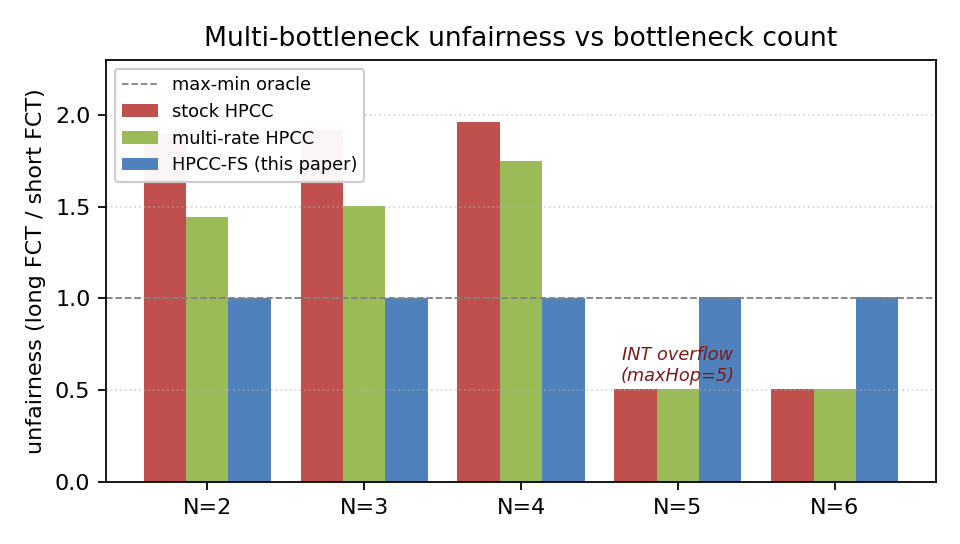
\includegraphics[width=\columnwidth]{fig_nsweep.png}
\caption{Multi-bottleneck unfairness vs bottleneck count $N$. \hpccfs is flat $\approx 1.0$
across the entire sweep; stock and multi-rate HPCC fail at $N \le 4$ and break at $N \ge 5$
(INT-overflow regime).}

\label{fig:nsweep}
\end{figure}

Stock and multi-rate HPCC are starved across $N = 2$--$4$ (penalty $1.90$--$1.96\times$ for stock,
$1.44$--$1.75\times$ for multi-rate), then break entirely at $N \ge 5$, where the per-hop INT
record overflows the \texttt{maxHop} cap (the apparent $0.51\times$ there is the overflow artifact,
not a real allocation). \hpccfs is flat at $1.003$--$1.007\times$ across the entire sweep ---
hop-count-independent by construction, since its single fair-rate field does not grow with path
length. HPCC-PINT, carrying one compressed utilization field, inherits load-based control and still
suffers ${\sim}1.8\times$ ($1.77$--$1.88\times$) --- the fix requires a fair-share signal,
not a smaller INT footprint. All \hpccfs runs have zero PFC events.

\subsection{The failure spans our evaluated stack}
\label{sec:endemic}

Is multi-bottleneck unfairness HPCC-specific? We ran every deployable RDMA scheme in our stack on
the same benchmark, with harness parity to the original HPCC evaluation (window-based schemes keep
their window; DCQCN, TIMELY, and DCTCP run windowless exactly as in their reference
configurations). Table~\ref{tab:endemic}: every scheme \emph{in our evaluated stack} is unfair to the
multi-bottleneck flow and worsens with bottleneck count --- DCQCN worst at $N{=}4$
($2.32\times$). HPCC is the norm here, not an outlier; only the RCP mode reaches max-min, and only HPCC and
the RCP mode hold zero PFC. Untested controllers (PowerTCP, Bolt, On-Ramp, Swift) are outside
the claim; a same-benchmark comparison is future work.

\begin{table}[t]
\caption{Unfairness ratio and PFC pauses on the parking lot: every deployable scheme fails
multi-bottleneck max-min; all worsen with $N$.}
\label{tab:endemic}
\centering\small
\begin{tabular}{lrrrr}
\toprule
scheme & $N{=}2$ & $N{=}3$ & $N{=}4$ & PFC \\
\midrule
DCQCN & $1.70\times$ & $1.90\times$ & $2.32\times$ & 6--34 \\
TIMELY & $1.83\times$ & $1.96\times$ & $2.01\times$ & 72--156 \\
DCTCP & $1.61\times$ & $1.72\times$ & $1.78\times$ & 256--280 \\
HPCC & $1.90\times$ & $1.92\times$ & $1.96\times$ & 0 \\
\hpccfs & $\mathbf{1.003\times}$ & $\mathbf{1.003\times}$ & $\mathbf{1.005\times}$ & 0 \\
\bottomrule
\end{tabular}
\end{table}

\subsection{When max-min is the objective: ring-collective coflow JCT}
\label{sec:jct}

Collective communication motivates multi-bottleneck fairness: a step completes only when its
\emph{slowest} flow completes (JCT $=$ max FCT), and the slowest flows are precisely the
cross-pod, multi-bottleneck ones stock HPCC starves. We run a 16-flow ring coflow --- the
traffic of one communication phase of a ring allreduce (each host sends 50 MB to its ring
successor: 4 inter-pod, 4 intra-pod, 8 same-edge segments); a full allreduce chains $2(N{-}1)$
such phases, so per-phase gains compound --- over all hosts of the $k{=}4$ fat-tree, across the
same five ECMP hash seeds. \hpccfs cuts JCT by $19.5$--$22.7\%$ (mean $21.4\%$) at \emph{every}
seed, and makes it nearly placement-invariant ($17.9$--$18.0$ ms across seeds, vs.\ stock's
$22.3$--$23.3$). Adding eight 2 MB
background flows leaves the JCT gain intact ($+20.6\%$ mean) and speeds the background flows
up ${\sim}3\times$ ($0.9$--$1.3$ vs $2.2$--$4.3$ ms): under near-winner-take-all dynamics a
short flow's fate is a placement lottery; max-min removes it. A header-size control rules out the confound of \hpccfs's smaller INT record: re-running
the coflow with the RCP class padded to stock's 42-byte layout (\S\ref{sec:integration}
transport, all flows FS) still gives $19.0$ ms vs stock's $23.3$ --- $18\%$ under
byte-identical headers, vs $23\%$ with the 8-byte field. The gain is fairness, not header
thinness. The 8-flow ECMP workload, read as a coflow, shows the same: makespan improves
$9.8$--$26.5\%$ across seeds.

\subsection{Structurally different topologies}

\begin{figure}[t]
\centering
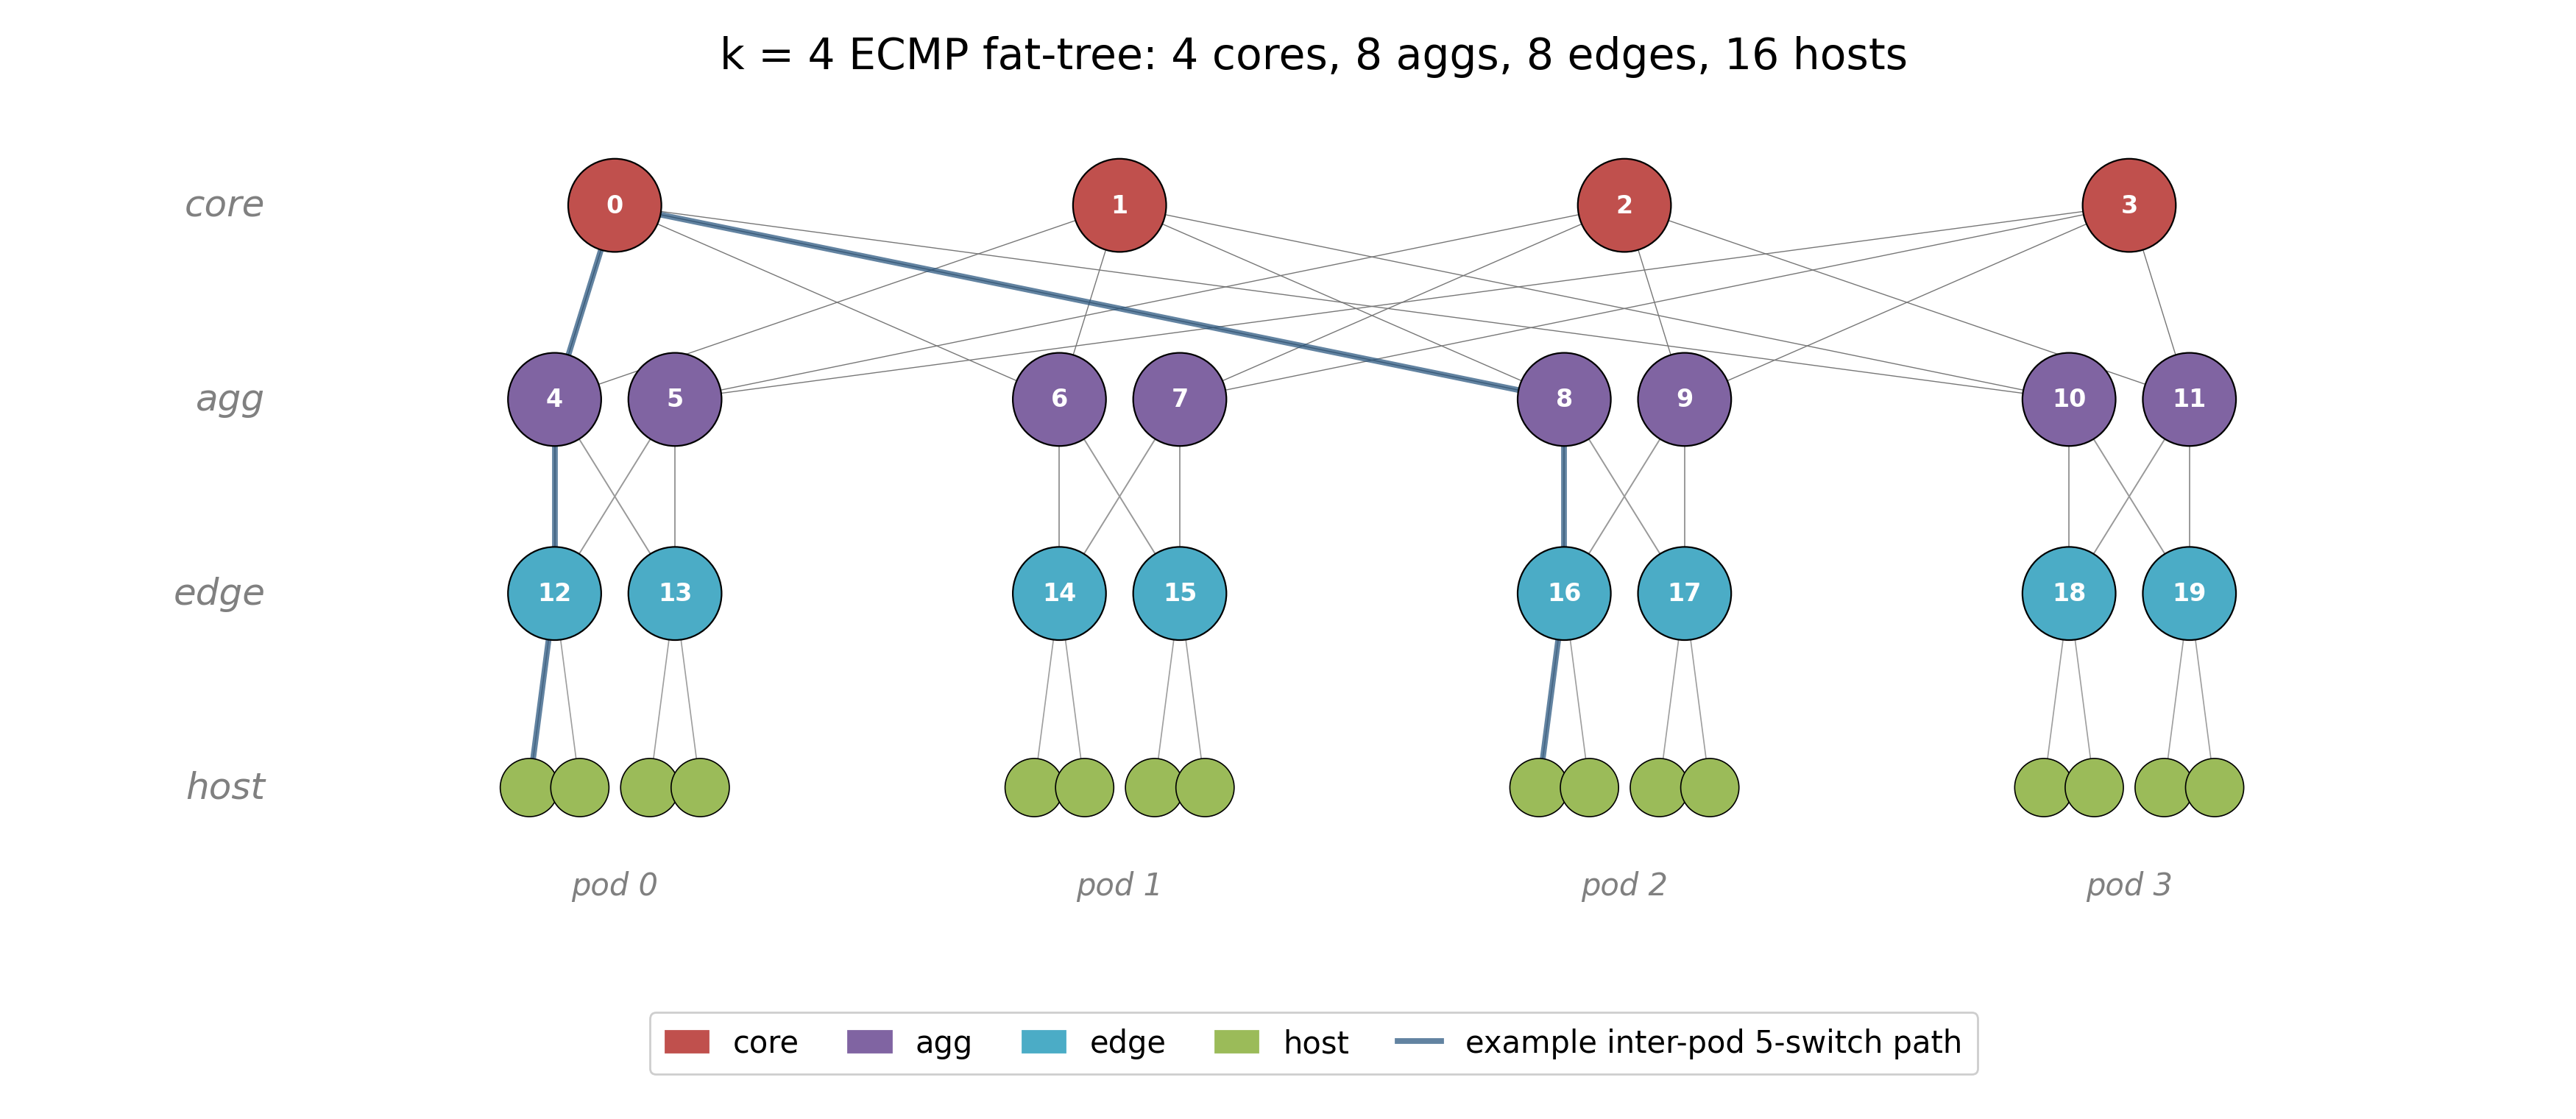
\includegraphics[width=\columnwidth]{fig_topo_fattree.png}
\caption{The $k=4$ ECMP fat-tree (4 cores, 8 aggs, 8 edges, 16 hosts in 4 pods); the highlighted
line is a representative inter-pod 5-switch path. The tree-fabric topology (unique shortest
paths, no ECMP) is described in the text.\label{fig:topo-ft}}
\label{fig:topos}
\end{figure}

\paragraph{Tree fabric (3-tier, no ECMP).} A 3-tier tree with unique shortest paths (15 nodes;
25 Gbps inter-switch, 100 Gbps host; Figure~\ref{fig:topos}). Stock penalty
$1.36\times$, \hpccfs $\mathbf{1.003\times}$, PFC $= 0$.

\paragraph{$k = 4$ fat-tree (with ECMP).} The canonical fat-tree (20 switches + 16 hosts;
Figure~\ref{fig:topo-ft}), hash-based ECMP; 4 inter-pod (5-switch) plus 4 intra-pod (3-switch)
flows. On the \emph{oracle-normalized penalty} (long-path vs.\ short-path slowdown, each
against the max-min oracle, removing placement effects): stock $1.34\times$, \hpccfs
$\mathbf{1.001\times}$. The \emph{raw} long/short ratio stays ${\sim}1.32\times$ under
\hpccfs --- not CC unfairness but placement: ECMP hashes some flows onto under-loaded cores,
inflating the raw ratio for any controller. PFC $= 0$ for both. Once placement is normalized
away, \hpccfs removes the multi-bottleneck penalty; path-min aggregation is path-invariant,
so ECMP needs no design changes. \emph{Hash-seed sensitivity.} Because a single deterministic run fixes one placement, we
re-ran the workload across \emph{twenty} ECMP hash seeds (an additive
\texttt{ecmp\_seed\_offset} knob shifts every switch's hash seed; the default preserves stock
behavior), reporting the mean-long/mean-short raw ratio. Under stock HPCC that ratio varies
$0.96$--$1.40\times$ across seeds (mean $1.14$) \emph{with no change to the congestion
controller} --- direct evidence that the raw spread is placement-dominated. Under \hpccfs the
mean is $1.04$ and the median $1.001$: fifteen of twenty seeds sit within $3\%$ of parity,
and the five residuals ($1.16$--$1.33\times$) are placements whose hash collides the long
flows onto shared cores, where equal FCTs are not the oracle allocation either. At the default
seed the contended case drops $1.338\times \to 1.001\times$. The oracle-normalized
conclusion is seed-robust (\texttt{run\_ecmp\_seeds.py} in the artifact).

\subsection{Robustness across asymmetric workloads}

\begin{figure}[t]
\centering
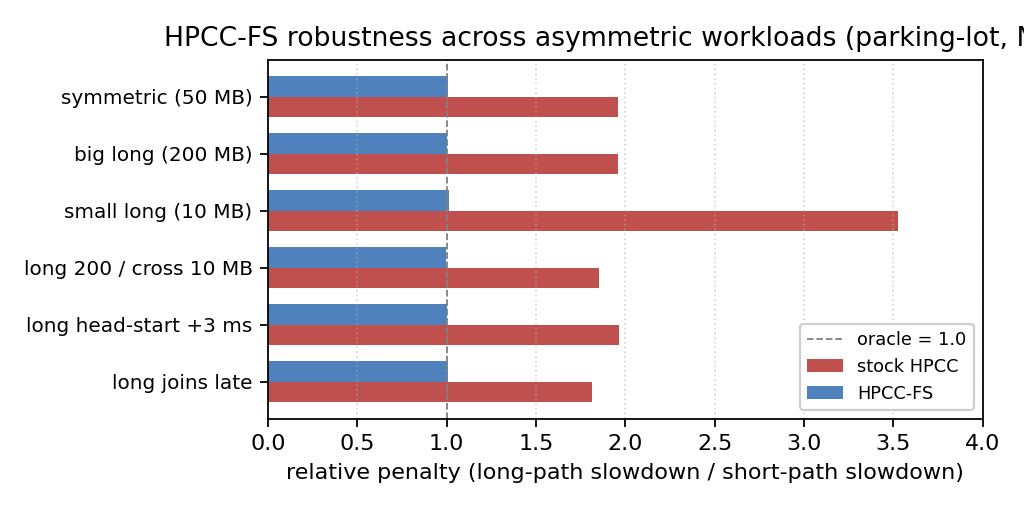
\includegraphics[width=\columnwidth]{fig_robustness.png}
\caption{Robustness across asymmetric-size and staggered-start variants at $N=4$. \hpccfs is
within $1.0 \pm 0.012$ across all six scenarios, including the small-long worst case where
stock reaches $3.53\times$.}

\label{fig:robustness}
\end{figure}

Across six perturbations (Figure~\ref{fig:robustness}), \hpccfs holds within $1.0 \pm 0.012$.
The worst stock case (small multi-bottleneck flow, $3.53\times$ penalty) drops to $1.012\times$.

\emph{Start-time jitter.} Jittering all five starts by $U[0,1]$\,ms (five seeds): stock
$1.96$--$1.99\times$, \hpccfs $1.008$--$1.017\times$. On the $N{=}1$ control the pairwise
spread persists at $1.10$--$1.39\times$ across $10\,\mu$s--$5$\,ms offsets with its
\emph{direction} flipping by arrival order --- the $\eta$-hold lottery, not synchronization ---
while \hpccfs equalizes the pair at every offset.

\subsection{Heterogeneous and dynamic contention}
\label{sec:hetero}

The uniform one-competitor parking lot is deliberately minimal, so we stress its assumptions
(Table~\ref{tab:hetero}; \texttt{run\_stress\_matrix.py}): heterogeneous capacities, unequal
competitor counts, two overlapping multi-bottleneck flows, and cross-flow churn. Each flow is
scored against a generic event-driven progressive-filling oracle on the actual topology and
schedule. A ratio alone can mask a uniform miss, so the table reports both the
\emph{generalized unfairness} (worst-long / best-flow $P_i$, reducing to the headline ratio in
the uniform case) and the absolute per-flow range of $P_i$.
Stock HPCC's unfairness grows with contention richness --- worst with two overlapping long
flows ($2.87\times$) and churn ($2.23\times$), its $P_i$ scattered $0.41$--$1.34$ (some flows
racing ahead of their oracle share while the longs lag) --- while \hpccfs holds
$1.001$--$1.007\times$ with $P_i \in [1.05, 1.13]$: \emph{every} flow lands within
$5$--$13\%$ of its own oracle FCT, a uniform convergence overhead, and mean bottleneck
utilization is \emph{higher} than stock in all four scenarios ($0.65$--$0.78$ vs
$0.51$--$0.70$). PFC $= 0$ everywhere; $4$--$8\times$ RTT spreads applied to the mode itself
leave the ratio at $1.003$--$1.008\times$. Jointly stressing the mode --- churn plus a
$4\times$ RTT spread plus $d$ misconfigured $4\times$ too small, at once --- leaves the ratio
at $1.000\times$ while the absolute $P_i$ rise to $1.21$--$1.39$: the compound stress costs
uniform slowdown, which the absolute metric exposes and the ratio alone would hide
(\texttt{run\_round3.py}). (INT admits only the discrete rates $\{25,50,100,200,400\}$
Gbps; heterogeneity is exercised within that set.)

\begin{table}[t]
\caption{Beyond the uniform parking lot: generalized unfairness and the absolute per-flow
range of oracle-relative FCT $P_i$. \hpccfs holds ${\approx}1.0\times$ with every flow within
$5$--$13\%$ of its oracle FCT; PFC $= 0$ throughout.}
\label{tab:hetero}
\centering\small
\begin{tabular}{lcccc}
\toprule
 & \multicolumn{2}{c}{stock HPCC} & \multicolumn{2}{c}{\hpccfs} \\
\cmidrule(lr){2-3}\cmidrule(lr){4-5}
scenario & unf. & $P_i$ range & unf. & $P_i$ range \\
\midrule
hetero cap.\ [25,50,25,100]\,G & $1.82\times$ & $0.64$--$1.16$ & $\mathbf{1.003\times}$ & $1.06$--$1.06$ \\
unequal comp.\ [3,1,2,1] & $1.41\times$ & $0.84$--$1.18$ & $\mathbf{1.001\times}$ & $1.06$--$1.06$ \\
two overlapping longs & $2.87\times$ & $0.41$--$1.19$ & $\mathbf{1.007\times}$ & $1.05$--$1.06$ \\
cross-flow churn & $2.23\times$ & $0.60$--$1.34$ & $\mathbf{1.002\times}$ & $1.06$--$1.13$ \\
\bottomrule
\end{tabular}
\end{table}

\subsection{Ablation: windows must scale with the fair rate}
\label{sec:ablation}

\hpccfs defaults to rate-only operation --- the per-flow window cap is disabled
(\S\ref{sec:design}). Table~\ref{tab:window} shows why, and shows the constraint is narrower
than ``no windows'': re-enabling HPCC's \texttt{var\_win} window degrades the penalty to
$1.5$--$2.5\times$, worsening with path length, because that window is sized from the NIC line
rate rather than the smaller multi-hop bottleneck path. The problem is the window's
\emph{scale}, not windowing itself: a canonical-RCP endpoint that sizes its window from the
adopted fair rate, $\mathit{cwnd} = R \cdot \mathrm{baseRTT}$ (the \texttt{fs\_rcp\_window}
knob), matches rate-only fairness while bounding in-flight data per flow --- a hard cap must
simply track $R$, not the NIC.

\begin{table}[t]
\caption{Window ablation: the NIC-scaled window breaks fairness; a fair-rate-scaled canonical RCP window preserves it (all zero PFC).}
\label{tab:window}
\centering
\small
\begin{tabular}{rccc}
\toprule
$N$ & rate-only (default) & NIC-scaled window & $cwnd = R \cdot \mathrm{RTT}$ \\
\midrule
2 & $\mathbf{1.003\times}$ & $1.50\times$ & $\mathbf{1.004\times}$ \\
3 & $\mathbf{1.003\times}$ & $2.00\times$ & $\mathbf{1.004\times}$ \\
4 & $\mathbf{1.005\times}$ & $2.49\times$ & $\mathbf{1.006\times}$ \\
\bottomrule
\end{tabular}
\end{table}

\subsection{Parameter sensitivity}
\label{sec:sensitivity}

We use the standard RCP defaults ($\alpha = 0.4$, $\beta = 0.226$) untouched. Sweeping each
parameter one at a time at $N = 4$ --- $\alpha \in [0.2, 0.6]$, $\beta \in [0.1, 0.4]$, startup
$R_0/C \in [0.25, 1.0]$, $\mathit{minRate} \in [100, 2000]$ Mb/s --- the penalty stays within
$[1.004, 1.008]\times$ with zero PFC throughout (even $R_0 = C$: the \texttt{m\_minRate} sender
start absorbs the first interval). Within this benchmark family the RCP parameters are not
load-bearing (\S\ref{sec:hetero} adds a three-factor joint stress). The control
interval $d$ tolerates misconfiguration asymmetrically: at $2$--$4\times$ too large, or
$2\times$ too small, the penalty stays $1.003$--$1.011\times$; at $4\times$ too small it
degrades to $1.212\times$ (updates outrun the feedback loop) --- still far below every baseline,
and PFC stays zero throughout.

\subsection{Queueing and PFC}
\label{sec:queue}

For context, every run uses the validated HPCC buffer model: 4 MB shared buffer with dynamic
PFC thresholds, ECN marking $k_{\min}/k_{\max}/p_{\max} = 100\,\mathrm{KB}/400\,\mathrm{KB}/0.2$
at 25 Gbps ($400/1600$ KB at 100 Gbps), 1000 B payload, $1$--$2\,\mu$s link delays. With the
smoothed startup (\S\ref{sec:startup}), \hpccfs produces \textbf{zero PFC events} on
every workload in the $N$-sweep and the robustness matrix. ECN marking remains; queue length is
bounded (peak ${\approx}46$ KB at $N=4$, versus ${\approx}118$ KB for stock HPCC on the same
workload); no flow loss. Do-no-harm holds throughout: the \hpccfs additions (implementation
name \texttt{HPCC-FS}, \texttt{cc\_mode 11}) only add code, and stock \texttt{cc\_mode 3}
smoke tests and $N$-sweep outputs are byte-identical to the pre-change baseline.

\subsection{High fan-in and idle-port staleness}
\label{sec:fanin}

Two stress cases target the event-driven update rule itself (\texttt{run\_round3.py}).
\emph{Incast fan-in:} $S$ senders to one 25 Gbps receiver link, 200 KB each,
$S \in \{3, 8, 16, 32, 64\}$. With the conservative 1 Gbps sender start, \hpccfs is
PFC-free through $S{=}32$ and there completes ahead of stock HPCC ($2.13$ vs $2.23$ ms); at
$S{=}64$ its first-interval overshoot leans on PFC (${\sim}4$k pauses vs.\ HPCC's 128) at
comparable FCT, and an aggressive 8 Gbps start triggers PFC from $S{=}32$. Extreme fan-in is
where stock HPCC's per-packet INT shines, and a measured boundary of the rate mode ---
latency-critical incast classes belong on stock HPCC (\S\ref{sec:scope}).
\emph{Idle-port staleness:} $R$ updates only on dequeue, so a port that goes idle freezes its
last $R$. We congest a port with four flows, let it idle for $g \in \{0.1, 1, 10, 100\}$ ms,
then release a single 1 MB probe: its FCT is $0.373$ ms at \emph{every} gap --- faster than a
fresh port's $0.713$ ms ($R_0 = C/2$ ramp) --- because the drain tail's final dequeues carry
$R$ back to ${\approx}C$ before the port empties --- the frozen value is benign, and no
aging term is needed in the evaluated regimes.

\subsection{HPCC's home turf: competitive FCT, lower queue}
\label{sec:cost}

What does the RCP mode cost on \emph{single}-bottleneck workloads --- HPCC's home turf? We
measure the validated incast benchmark (3 senders $\to$ 1 receiver over 25 Gbps; 12 flows,
100--400 KB), sweeping the sender's startup rate:

\begin{table}[t]
\caption{HPCC's home turf (single-bottleneck incast). \hpccfs holds far less queue than HPCC at
every startup, and a moderate startup also matches or beats HPCC's FCT. The same startup leaves
the multi-bottleneck fairness headline unchanged ($1.003$--$1.004\times$, PFC $= 0$).}
\label{tab:hometurf}
\centering
\small
\begin{tabular}{lccc}
\toprule
 & mean FCT & tail FCT & peak queue \\
\midrule
HPCC & 258.6 $\mu$s & 459.8 $\mu$s & 143 KB \\
\hpccfs (startup 1 Gbps) & 297.5 $\mu$s & 490.3 $\mu$s & \textbf{64 KB} \\
\hpccfs (startup 5 Gbps) & 271.2 $\mu$s & 464.3 $\mu$s & \textbf{49 KB} \\
\hpccfs (startup 8 Gbps) & \textbf{242.0 $\mu$s} & \textbf{416.8 $\mu$s} & \textbf{38 KB} \\
\bottomrule
\end{tabular}
\end{table}

Two things stand out (Table~\ref{tab:hometurf}): \hpccfs holds far less queue than HPCC at
every startup ($38$--$64$ KB vs $143$ KB), and HPCC's only lead --- FCT at the conservative
1 Gbps startup (${\sim}15\%$) --- closes and reverses at 8 Gbps (242 vs 259 $\mu$s at
one-quarter the queue, zero PFC). The 8 Gbps point leaves the multi-bottleneck headline
undisturbed ($1.003$--$1.004\times$, PFC $=0$); the headline runs use 1 Gbps. On these
workloads the fairness mode costs little-to-no FCT and holds less queue. Before the first
fair-rate ACK a sender emits at most $\mathit{startup} \times \mathrm{baseRTT}$
(${\approx}2.7$ KB at 1 Gbps), and the $cwnd = R \cdot \mathrm{RTT}$ variant
(\S\ref{sec:ablation}) restores a hard per-flow cap thereafter; the fan-in limit of this
startup bound is measured directly in \S\ref{sec:fanin}. \hpccfs still lacks HPCC's
per-hop, window-bounded reaction --- \S\ref{sec:fanin} measures the $S{=}64$ boundary ---
and recovering it while keeping fairness is the hybrid's target (\S\ref{sec:discussion}).

\subsection{Per-flow rate trace, before vs after}

\begin{figure*}[t]
\centering

\includegraphics[width=0.94\textwidth]{fig_rate_trace.png}
\caption{Per-flow goodput at $N = 4$, stock HPCC (left) vs \hpccfs (right). Stock collapses the
long flow to ${\sim}0.4$ Gbps while cross flows hold ${\sim}23$ Gbps for 18 ms (winner-take-all).
\hpccfs converges all five flows to within $5\%$ of the max-min fair share (12.5 Gbps) in
${\sim}0.6$ ms and to within $1\%$ by ${\sim}2.3$ ms.}

\label{fig:rate-trace}
\end{figure*}

The before-vs-after rate trace (Figure~\ref{fig:rate-trace}) is the cleanest qualitative
result: collapse to ${\sim}0.4$ Gbps under stock, lock-in at fair share under \hpccfs.

\subsection{Scope of the headline claim}
\label{sec:scope}

The ${\approx}1.0\times$ headline is a statement about the \emph{congestion-control component}
of multi-bottleneck unfairness on contention benchmarks --- not a claim of universal FCT
improvement on production workloads. Five first-class limits. (i)~\emph{Mixed short-flow
workloads} do not exhibit the penalty we target: under a WebSearch distribution stock HPCC's
oracle-normalized penalty is already $1.001\times$ (\hpccfs: $0.581\times$), and on mean slowdown
\hpccfs trades ${\sim}15\%$ off multi-bottleneck flows for ${\sim}45\%$ on short paths.
Short-flow-FCT
workloads~\cite{montazeri2018homa,alizadeh2013pfabric} may prefer stock HPCC; max-min matters
when multi-bottleneck flows gate a job (\S\ref{sec:jct}). Selecting the mode per service is
possible only with per-class link or telemetry isolation --- \S\ref{sec:integration} shows an
unsliced shared port serves neither class --- so the deployment unit is a fabric, or a slice of
one, dedicated to traffic that wants max-min; this is not a global replacement.
(ii)~\emph{Fabric scale}: our $k = 6, 8$ scaling workload does not form persistent
inter-pod contention (both penalties ${<}1$), so we added a \emph{saturating} $k{=}6$ case
--- 108 identical 20 MB inter-pod flows, every stage at capacity under ECMP
(\texttt{run\_scale\_saturate.py}): coflow makespan $42.9 \to 35.9$ ms ($-16\%$), Jain
$0.91 \to 0.93$ (residual spread is ECMP placement for both), PFC $= 0$ at 45 switches;
$k{=}8$ at saturation is future work. (iii)~\emph{ECMP placement}: a raw ${\sim}1.3\times$ long/short spread from hash placement
remains; \hpccfs removes the CC component only. (iv)~\emph{Coexistence}: the modes do not share a link fairly even under DRR reservation
(\S\ref{sec:integration}); \hpccfs is a fabric-wide mode. (v)~\emph{Extreme fan-in}: at
$S{=}64$ incast the rate mode leans on PFC where stock HPCC barely does
(\S\ref{sec:fanin}).

% ============================================================================
\section{Related Work}
\label{sec:related}
% ============================================================================

\paragraph{Datacenter transport.} DCTCP~\cite{alizadeh2010dctcp}, DCQCN~\cite{zhu2015dcqcn},
TIMELY~\cite{mittal2015timely}, and Swift~\cite{kumar2020swift} trade buffering for latency via
ECN- and delay-based control; Homa~\cite{montazeri2018homa} and pFabric~\cite{alizadeh2013pfabric}
prioritize short flows; HPCC~\cite{li2019hpcc} drives control from per-hop INT, with
On-Ramp~\cite{liu2021onramp} and PowerTCP~\cite{addanki2022powertcp} extending the precise-signal
philosophy. Across this line the target is single-bottleneck FCT, tail latency, or queueing;
\S\ref{sec:endemic} shows every member we evaluate fails multi-bottleneck fairness.

\paragraph{In-network telemetry.} INT~\cite{kim2015int} lets the data plane stamp per-hop state into
packets on programmable pipelines, and HPCC was among the first to drive congestion control directly
from it. The cost is header overhead, which later work minimizes: HPCC-PINT~\cite{yang2020pint}
compresses the per-hop record into a single probabilistic field, and Poseidon~\cite{wang2023poseidon}
restructures INT-based control for deployability on commodity hardware. \hpccfs continues this
minimal-telemetry direction but changes \emph{what} the field carries: an explicit fair
\emph{rate}, min-aggregated along the path --- one 64-bit field, like PINT, yet a decision
rather than a measurement.

\paragraph{Explicit-rate and switch-assisted control.} Having the switch compute and return a sending
rate is a classic idea. ATM ABR explicit-rate schemes such as ERICA~\cite{kalyanaraman2000erica}
computed a fair share per port decades ago; XCP~\cite{katabi2002xcp} decomposed switch feedback into
separate efficiency and fairness controllers; and RCP~\cite{dukkipati2008rcp} reduced this to a single
fair-rate scalar per link with no per-flow state, packet-stamped, with senders taking the path minimum.
RCP is the closest mechanism to ours: \hpccfs adopts its update rule but situates it as a \emph{minimal
fairness signal injected into an existing INT load-signaling system} rather than a standalone protocol,
keeping HPCC's single-rate sender and per-hop transport. Prior RCP work established
explicit-rate fairness in general fabrics; what had not been measured is whether deployed
INT-based RDMA stacks exhibit the multi-bottleneck gap, and whether a telemetry-carried fair
rate closes it \emph{inside} such a stack --- that measurement is this paper's contribution. \hpccfs's per-port update and path-min aggregation \emph{are} RCP's; the endpoint differs
(rate-only by default; the canonical window performs equally, Table~\ref{tab:window}), the
control interval is a fabric constant, updates are event-driven, and the port applies
$R_0 = C/2$ and a floor. Over deploying RCP as a separate protocol, \hpccfs adds packaging,
not control: one field on the INT transport already running, a byte-identical stock path,
per-mode selection --- no second stack.

\paragraph{In-switch fairness.} Fair queueing~\cite{demers1989fq}, DRR~\cite{shreedhar1995drr},
CSFQ~\cite{stoica1998csfq}, and AFD~\cite{pan2003afd} enforce fairness in the scheduler;
\S\ref{sec:senderonly} shows scheduling alone does not correct window-limited INT senders.
\hpccfs instead \emph{advertises} one fair rate per port --- no per-flow tracking, no extra
queues --- implementable on the match-action pipelines~\cite{bosshart2014p4} INT already
assumes.

\paragraph{Closely related switch-assisted DC schemes.} Bolt~\cite{arslan2023bolt} accelerates
HPCC's loop with sub-RTT per-flow switch assistance, targeting tail latency and ramp-up ---
orthogonal to our objective: its feedback carries load/supply, not a fair share, so the
history argument of \S\ref{sec:senderonly} applies to its senders too; a faster load-signal
loop converges faster to the same equilibrium. We leave a head-to-head to future work.

% ============================================================================
\section{Discussion}
\label{sec:discussion}
% ============================================================================

\paragraph{Relation to HPCC, and a hybrid path.} \hpccfs inherits RCP's character --- fair,
low-queue --- without HPCC's single-flow precision (\S\ref{sec:cost}). A future hybrid caps HPCC
at the fair rate, $\min(\mathit{rate}_{\mathrm{HPCC}}, R)$; the obstacle is HPCC's NIC-sized
window (\S\ref{sec:ablation} suggests a fair-rate-scaled one).

\paragraph{Scaling and hardware.} At $k = 6, 8$ the fabric's $(k/2)^2$ cores spread
inter-pod flows so persistent contention does not materialize for our scaling workload (both
schemes' penalty ${<}1$; \hpccfs adds no overhead, 0 PFC); the saturating case is in
\S\ref{sec:scope}. On hardware we offer a mapping, not a prototype: three registers per port ($R$, timestamp, byte
snapshot); a dequeue-triggered fixed-point update with $1/C$ and $\beta/d$ precomputed (two
multiplies, two subtractions, a clamp); and a 64-bit compare-and-write path-min per packet. Each
piece has P4 precedent, but stage budget and dequeue-time queue-depth access are
switch-specific; a Tofino prototype remains future work.

\paragraph{Limitations.} Three topology families; in-sim baselines only (DCQCN, TIMELY, DCTCP,
multi-rate HPCC, PINT) --- no Bolt/PowerTCP re-implementation and no testbed; per-class
coexistence requires link or telemetry isolation we do not design (\S\ref{sec:integration}); the ECMP study is
a small controlled workload (though seed-swept), not a realistic mixed-size + ECMP combination.
All numbers come from one simulator --- but its control logic is the original HPCC
implementation with interface-level modernization only, verified end-to-end by reproducing the
original baselines, and the $N \le 4$ regime sits within the 5-hop INT budget by construction; a
belt-and-braces run on the unmodified legacy build remains future work; the result is
insensitive to the RCP parameters (\S\ref{sec:sensitivity}).

% ============================================================================
\section{Conclusion}
% ============================================================================

Multi-bottleneck unfairness spans every deployable RDMA scheme in our stack, and HPCC's
instance is a stable, RTT-independent, near-winner-take-all equilibrium (${\sim}2\times$;
$3.5\times$ for small flows; unchanged over $10\times$ longer backlogs). Six sender-side
corrections fail --- including an exact private mirror of RCP --- and so does per-flow fair
queueing under stock senders; a controlled fluid experiment shows why: with identical
observations, law, and epochs, privately held explicit-rate state still freezes arrival-order
asymmetry, while one shared per-link register erases that history. \hpccfs carries that
register's value in one INT field --- three words of mutable state per port --- reaching
penalty $1.005\times$, every flow within $5$--$13\%$ of its oracle FCT, with zero PFC in
every fairness experiment, rate-only or canonically windowed, converging sub-millisecond and
independent of path length, with the stock HPCC code path byte-for-byte unchanged.
Coexistence on a shared link fails even under a DRR reservation (\S\ref{sec:integration}):
the mode belongs on sliced telemetry or a separate fabric, not in free competition.

\bibliographystyle{IEEEtran}
\bibliography{paper}


\end{document}
